% !TeX spellcheck = en_US
% Chapter Template

\chapter{Background and related work} % Main chapter title

\label{chap:background} % Change X to a consecutive number; for referencing this chapter elsewhere, use \ref{ChapterX}

\lhead{Chapter \ref*{chap:background}. \emph{Background and related work}} % Change X to a consecutive number; this is for the header on each page - perhaps a shortened title

\section{Application under study}
\acf{OT} is a open-source simulation platform developed by the university of Applied Sciences in Frankfurt, Germany. It covers features like computer aided design and meshing and is also a physics simulation (having solvers for Finite Integration and PHREEC). The projects can be administered by a user and group management (see~\autoref{fig:ot-project}). Furthermore, all changes on a project are version-controlled. The application is designed in a way, that only a local thin-client needs to run on the users computer. After entering the login credentials (see~\autoref{fig:ot-login}), the client securely connects to a centralized service platform where the computation is made. The results and even the \ac{UI} information is sent back to the client application. This has the benefit, that also weak computers can run the application.

\begin{figure}[h]
	\centering
	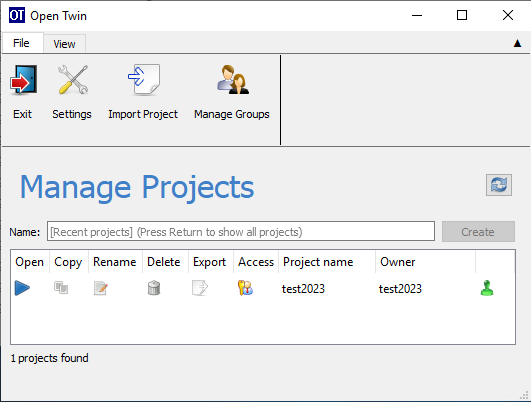
\includegraphics[width=.9\textwidth]{Figures/ot-project.png}
	\caption{The \ac{OT} project overview.}
	\label{fig:ot-project}
\end{figure}

\begin{figure}[h]
	\centering
	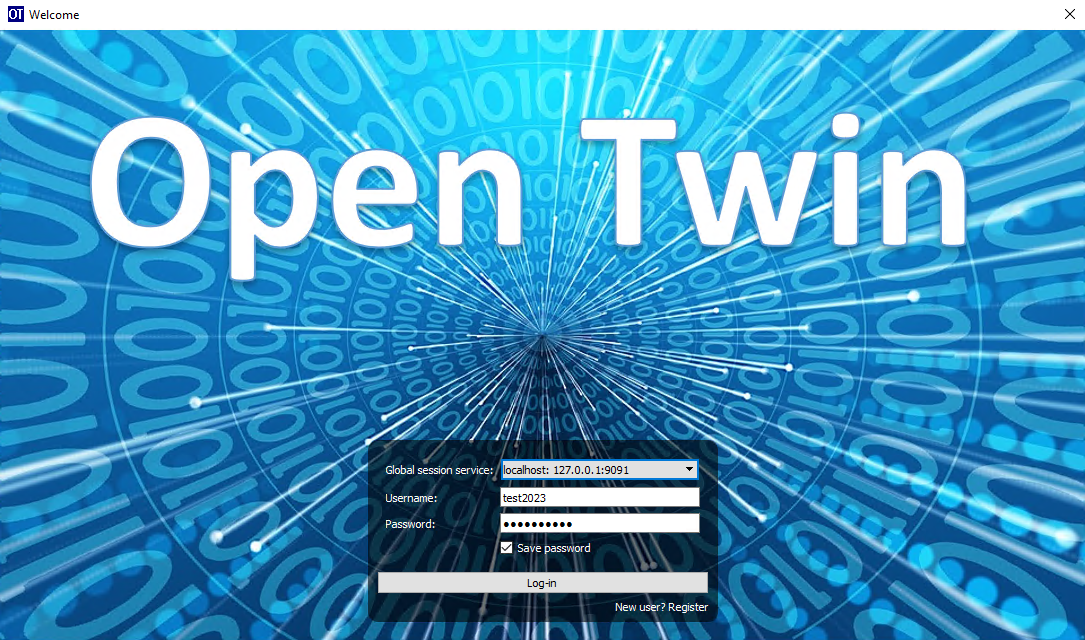
\includegraphics[width=.9\textwidth]{Figures/ot-login.png}
	\caption{The \ac{OT} login screen.}
	\label{fig:ot-login}
\end{figure}

\autoref{fig:ot-model} shows the application itself with a loaded project and a simple geometric model.
\begin{figure}[h]
	\centering
	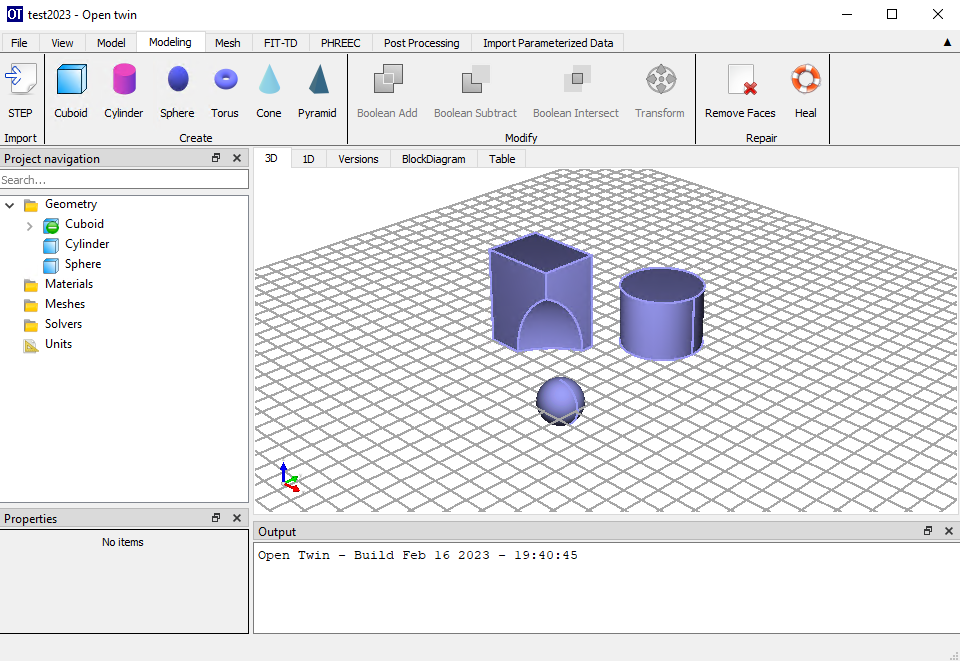
\includegraphics[width=.9\textwidth]{Figures/ot-model.png}
	\caption{A opened project inside \ac{OT} with a few created geometric models and subtracted computation.}
	\label{fig:ot-model}
\end{figure}

The development team consists of a small core team and several student groups during the semester.


\section{Baseline architecture}
\label{chap:background.baseline_architecture}
The current system design consists of multiple levels. It is a multi-process application based on the programming languages C++ and Rust. The source code is mainly aligned to be built on Microsoft \ac{Windows}. A port to Unix based systems is currently in work. Therefore parts of the code base are aligned for multiple system architectures already, but the application is not yet able to be compiled for Linux.

Each microservice of the application is included dynamically and linked as a \ac{DLL} file. For starting the microservice environment, a central executable (\enquote{open\_\ twin.exe}) is started with the corresponding arguments for the services (like the server's binding address, port numbers, and passwords) (see~\autoref{lst:ot-command}) and the path to the \ac{DLL} file itself. The UI front end, which is started by the user directly, is compiled in its own executable (\enquote{uiFrontend.exe}).

\begin{lstlisting}[language=sh, caption={Command line of Open Twin Service start}, label=lst:ot-command]
open_twin.exe GlobalSessionService.dll \
  "0" "127.0.0.1:8091" "tls@127.0.0.1:27017" "127.0.0.1:8092"
\end{lstlisting}

For conveniently running the services with all their necessary arguments, batch files were provided that read environment variables and convert them into runtime arguments for the service executable. Therefore, if the services are started locally, the user runs a batch file that sets up the environment for the network binding details, path to certificates and encrypted database credentials.

The system consists of the following micro services that are permanently accessible: \acf{GSS}, \acf{AUTH} and the database. The database is running on MongoDB\footnote{MongoDB:~https://www.mongodb.com/}. Another Service is the \acf{LSS} that spawns the so called compute services. Those are services for running the actual computation after opening a project that can dynamically spawn and exit. A partial list of compute services and their corresponding tasks can be found in \autoref{tbl:ot-compute-services}.
Each service runs in its own operating system process.

\begin{table}[h!]
	\centering
	\begin{tabular}{|l | p{.65\textwidth}|} 
		\hline
		Name & Task  \rule{-5pt}{2.6ex} \\
		\hline \rule{-3pt}{3ex}
		CartesianMeshService & If demanded, it converts a continuous geometry into a discrete Cartesian mesh. \\
		FITTDService & If demanded, it runs a solver algorithm for transle electromagnetic simulation based on the finite integration technique (FIT).\\
		KrigingService & If demanded, it runs a kriging interpolation of result data. \\ 
		LoggerService & A background service, that accepts logging messages from other services. \\ 
		ModelingService & Performs calculations for the creation, modeling and boolean combination of geometric data. \\ 
		PHREECService & If demanded, it runs simulation based on PHREEC. \\ 
		TetMeshService & If demanded, it meshes a form with an tetrahedral mesh.  \\ 
		VisualizationService & Runs the graphical calculations for displaying the geometric and data based results on the \ac{UI}.\\ 
		[1ex] 
		\hline
	\end{tabular}
	\caption{List of compute services and their corresponding tasks.}
	\label{tbl:ot-compute-services}
\end{table}


As shown in \autoref{fig:ot-network-communication-diagram}, the services can be separated by their network space. Not all services require a public available network address.
While \ac{GSS}, \ac{AUTH} and database are globally accessible via a fixed network address, the \ac{LSS} can theoretically run on a dedicated host and is only communicated to other parties after it has registered itself to the \ac{GSS}. The services, spawned by \ac{LSS} do not require a public address space either. All communication between the \ac{UI} front end and the compute services is achieved via a relay service and a web socket communication channel.

\begin{figure}[h]
	\centering
	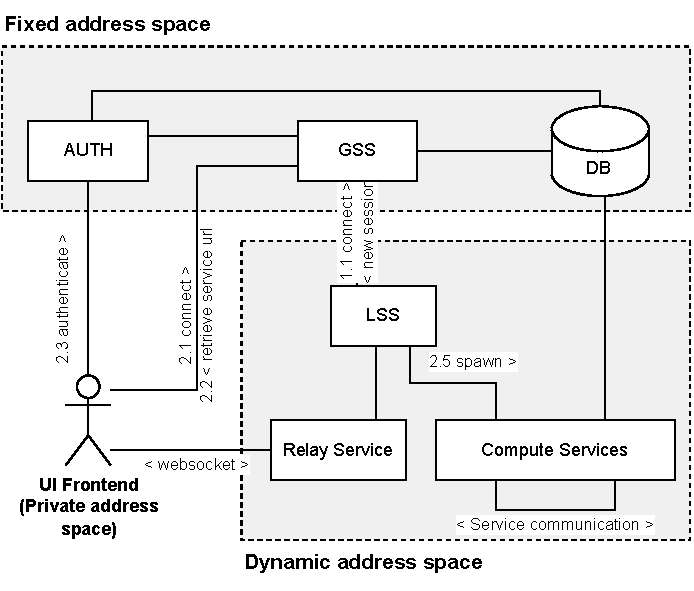
\includegraphics[width=0.7\textwidth]{Figures/opentwin-network-communication-diagram.pdf}
	\caption{Communication overview and service organization for \ac{OT} main services. In 1.1 the \ac{LSS} registers at \ac{GSS}. As soon as the \ac{UI} front end connects to the \ac{GSS}~(2.1), service information is exchanged~(2.2) and the user is authenticated~(2.3). As a consequence, the \ac{GSS} creates a new session and tells the \ac{LSS} to spawn new compute services. From now on the \ac{UI} front end communicates directly with the Compute services via the Relay Service over a web socket connection.}
	\label{fig:ot-network-communication-diagram}
\end{figure}


The whole process of the \ac{LSS} registration and connection of the \ac{UI} front end to the compute services is depicted in \autoref{fig:ot-network-communication-sequence}.
Once started, the user can login. In order to connect to the database, the following steps are performed:
\begin{enumerate}
\item The \ac{UI} front end requests further service information from the publicly available \ac{GSS}. The address for this service is provided by the user. The \ac{GSS} responds with \acp{URL} to the database and the \ac{AUTH}.
\item The \ac{UI} front end connects to the \ac{AUTH} using the authentication information provided by the user.
\item If the \ac{AUTH} replies with a positive authentication, the \ac{UI} front end connects to the database and lists the projects.
\item Once a project is opened or created, the \ac{UI} front end requests a new session from the \ac{GSS}. The \ac{GSS} replies with the connection \acp{URL} of the \ac{LSS}. The \ac{LSS} has been registered to the \ac{GSS} during its initialization.
\item The \ac{UI} front end then connects to the \ac{LSS} and requests a new session. As a result, the \ac{LSS} spawns new application service processes and replies with the respective service \acp{URL}.
\item From now on, the \ac{UI} front end communicates with the application services via the Relay service over a web socket.
\end{enumerate}

\begin{figure}[h]
	\centering
	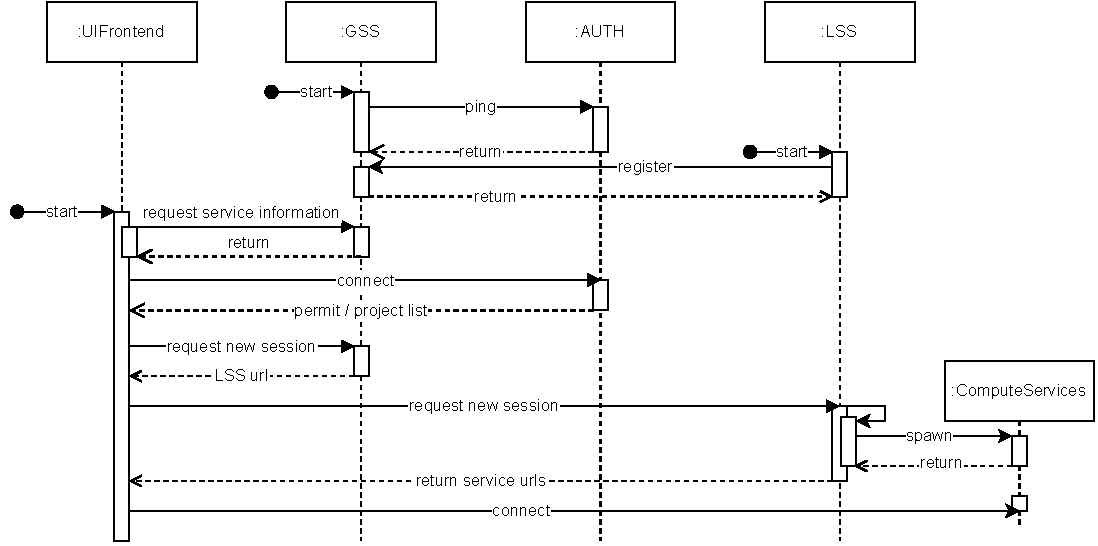
\includegraphics[width=0.98\textwidth]{Figures/opentwin-network-communication-sequence.pdf}
	\caption{Service initialization of \ac{OT} processes. In the beginning, the main services \ac{GSS}, \ac{AUTH} and an optional \ac{LSS} are initialized. While the \ac{GSS} checks the reachability of \ac{AUTH}, the \ac{LSS} registers itself at the \ac{GSS}. After starting the \ac{UI} front end, the service information is requested from a \ac{GSS} and the user is authenticated. Afterwards, the project list for the authenticated user is displayed. After opening a project, the \ac{UI} front end connects to the \ac{LSS} and requests a new session. As consequence, the \ac{LSS} spawns the compute services and connects them to the \ac{UI} front end via a Relay Service. (Ping messages are omitted.)}
	\label{fig:ot-network-communication-sequence}
\end{figure}

%The traffic between services is encrypted using \ac{mTLS} technology. While regular \ac{TLS} ensures the authenticity of the server by using Certificates and the chain of trust, it does not verify the identity of the client. This is the benefit of \ac{mTLS}. In \ac{mTLS}, both sides, client and server has to verify their identity by providing a certificate inherited from a common root authority.

% TODO: OpenGL -> file rename


% TODO: Section about "Containerization and/vs VM"
% TODO: Section about "Container & Container image"
% TODO: Einführung Containerd CLI tools (crictl, nerdctl, ctr <preinstalled>)
% TODO: ContainerD kann kein Build auf Windows - buildkit daemon is required, buildkit: only linux is supported (https://github.com/moby/buildkit) buildkitd is only available for Linux currently. 
% TODO: Container file == Container file definition of file type .Containerfile


\section{Network traffic encryption}
Each service of \ac{OT} offers two different channels for secure communication between services. One channel supports traditional one-way \ac{TLS}, while the other uses bidirectional \ac{mTLS}. The one-way \ac{TLS} channel is mostly used for checking the general health state of a service, while the two-way \ac{mTLS} is used for relevant application based communication.
In this section both encryption methods are briefly presented.

\subsection{Transport Layer Security}
\ac{TLS} is an cryptography extension mainly designed for providing security over \ac{HTTP}. The main goals of cryptography are confidentiality, integrity and authenticity between two communicating parties. This means, the communication on a network is kept secret between the two endpoints (Confidentiality), messages are not subject of manipulation (Integrity), and message exchanges are only allowed between authorized and trusted individuals (Authenticity). \ac{TLS} ensures the three traits by using certificates.

A simplified handshake of the \ac{TLS} protocol is depicted in \autoref{fig:tls-protocol}.
After sending the certificate from server to the client, the client validates the certificate based on the chain of trust. This means, it checks if the certificate was issued by a trusted root authority (so called \ac{CA}). Only if the authenticity of the server is ensured, the encryption key is exchanged in order to start an encrypted communication.

\begin{figure}[h]
	\centering
	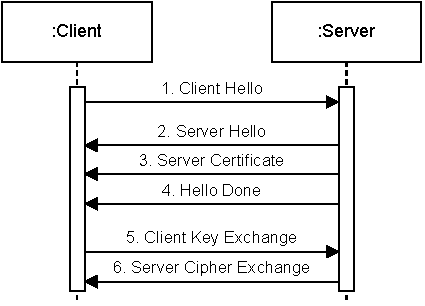
\includegraphics[width=0.55\textwidth]{Figures/tls.pdf}
	\caption{Simplified visualization of the \ac{TLS} handshake\cite{Rescorla.2018}. After initialization of the handshake (1,2), the server sends its certificate (3) and finishes with a message \enquote{Hello Done} (4). The client then validates the certificate and compares it against the chain of trust. Afterwards, the key exchange starts (5,6) to ensure an encrypted communication.}
	\label{fig:tls-protocol}
\end{figure}


\subsection{Mutual authentication}
The mutual authentication is adding another step to the one-way authentication. The application of it is used in \ac{mTLS} as extension of the classic \ac{TLS} protocol\cite{Rescorla.2018, HugoKrawczyk.2016}. Instead of just sending the server's certificate to the client, the client also sends a certificate to the server. Therefore, not only the authenticity of the server is ensured, but also of the client.

As can be seen in \autoref{fig:mtls-protocol}, compared to the \ac{TLS} handshake, the \ac{mTLS} handshake involves additional messages 5 and 6 for sending and validating the client's certificate.
Unlike with the server certificate, the client certificate is not validated against a publicly available root authority\cite{Cloudflare.20230309, Rescorla.2018}. Instead, the server acts as root authority, creates the client certificate and ships it with the application\cite{Cloudflare.20230309}.


\begin{figure}[h]
	\centering
	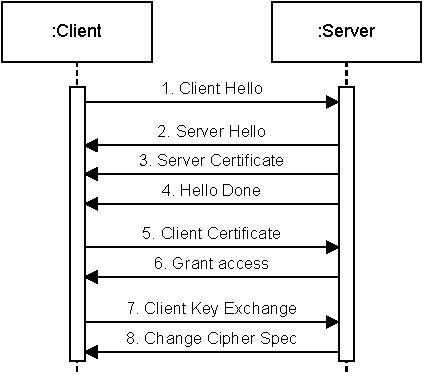
\includegraphics[width=0.55\textwidth]{Figures/mtls.pdf}
	\caption{Simplified visualization of the \ac{mTLS} handshake\cite{Cloudflare.20230309, Rescorla.2018}. After initialization of the handshake (1,2), the server sends its certificate (3) and finishes with a message \enquote{Hello Done} (4). The client then validates the certificate and compares it against the locally stored root authority. Afterwards, the client sends its certificate to the server (5). The server validates the client certificate against its local root authority and grants access to the service (6). Afterwards, the key exchange starts (7,8) to ensure an encrypted communication.}
	\label{fig:mtls-protocol}
\end{figure}

\subsection{Certificate creation}
For creation of certificates in the application landscape of \ac{OT}, CloudFlare's public key infrastructure toolkit \enquote{cfssl}\footnote{cfssl: https://cfssl.org/ or https://github.com/cloudflare/cfssl} is used.
For generating certificates with the toolkit, it is fed with a JSON file with subject information for the \ac{CSR}.

It contains information about the issuer, as well as the name and cryptography algorithm of the certificate.
Additionally, the client and server certificate that derive from the root \ac{CA} contain information for whitelisted hosts in their \ac{CSR} JSON file. If a host is not mentioned in the resulting certificate, requests from the corresponding host are rejected.
\autoref{lst:background.ca-csr} shows such a configuration with accepted host names in the form of a \ac{CSR}.

\begin{lstlisting}[label=lst:background.ca-csr, caption={Example of meta data in form of \ac{CSR} configuration. \enquote{CN} is the certificate name. \enquote{hosts} describes the accepted hostnames, \enquote{key} describes information about the cryptography algorithm, \enquote{names} contains meta data of the organization}]
{
  "CN": "OpenTwin",
  "hosts": ["localhost", "127.0.0.1"],
  "key": {
    "algo": "rsa",
    "size": 4096},
  "names": [{
    "O": "Frankfurt University of Applied Sciences"
  }]
}
\end{lstlisting}


\section{Problem statement}
Even though, the application is clearly based on a microservice architecture and it is able to run on a distributed system, it is not designed for an automated cluster yet.
It consists of multiple processes where many of them have to run on the same system and need a full working operating system as baseline.  % TODO(THOMA): DAS MUSS JA NICHT SEIN - "Have to run on same system."
Containerization of the system has never been tested and needs to be introduced. 
First, the cluster engine needs to be set up for \ac{Windows} compute nodes to allow \ac{Windows} containers to run inside the cluster. Additionally, it needs to have full network capabilities as well as inter connectivity between the several services.
Next, the application needs to run inside containers. Therefore, container images must be created and provided for the cluster engine. 
Additionally, the automatic extension of services requires communication between the cluster orchestration management and the applications running on the nodes. A feature that needs to be introduced later on.

Regarding logging, while the front end application does, the microservices currently do not produce log files. Instead, only a few sub processes write the information on its standard output stream. In some cases, the error information given by exceptions is dropped.
Furthermore, proper exit codes in error cases are not returned. That is, if the application exits there is currently no way to detect if the process terminated normally or crashed as part of an error.

\section{Limitations}
Due to the limited amount of time, not all code changes are applied. On the one hand, this involves the adaption for automatic extension of services. On the other hand, it implies the changes required to make the application more fault-tolerant. The changes that would be necessary, would be too extensive. Therefore, they are only made to the main processes.

As a first case study, the application is not fully containerized. Since the network connectivity is known to cause troubles in \ac{Windows} container networks, there is more investigation required later on. As part of this study, only the main services are containerized and the cluster is set up to investigate the behavior in cluster environments. The actual distribution of an full functional cluster network can be part of further studies later on.

\section{Related Work}
